\chapter{Angles, Joints and Hands}
\label{C:angles-joints-hands}

This next chapter discusses the development of a model to predict motion of a human hand. To understand the model and some of the implementation choices, it is necessary to understand the anatomy of the hand, and how the many degrees of freedom of the hand can be represented (paramaterized). This chapter discusses the different ways to parameterize angles, 3D rotations, and collections of many joints. It also introduces some loss functions for training neural networks where the input and output are angles.

\section{Representing Angles}

In toplogical terms, an angle is a point on the unit circle, aka the 1-sphere $S^1$. In the context of 3D rotations, an angle is a rotation around a single axis. We typically use either of two representations for angles: A single number or a 2D unit vector.

Representing an angle as a single number (in either radians or degrees) is the most common representation. It is simple and addition between angles represented in this way is well defined.

The other representation is the unit vector representation. In this representation, an angle $a$ is represented by a 2D unit vector $v$
\begin{equation}
    v = \begin{bmatrix}x \\ y\end{bmatrix} = \begin{bmatrix}\cos{a} \\ \sin{a}\end{bmatrix}
\end{equation}.
This representation is useful for neural network implementations for two reasons:
\begin{enumerate}
    \item The dot product between two unit vectors is equal to the cosine of the angle between them. This means that the dot product between two unit vectors can be used as a measure of the similarity between two angles.
    \item Linear interpolation between two unit vectors gives a vector which has the same angle as the linear interpolation between the two angles. This means that if we re-normalize the vector, we get a unit vector which represents the same angle as the linear interpolation between the two angles.
\end{enumerate}

Using the unit vector representation also makes it simpler to define the \textit{circular mean} operation (which will be used later in \Cref{C:hand-model})

\subsection{Circular mean}
\label{ss:circ-mean}

Take for example two angles in radians, $a = 0$ and $b = 2\pi-1 \approx 5.28$. They represent angles 1 radian apart, but naively computing the midpoint between them would give $\pi-0.5 \approx 2.64$, which is not correct. The correct answer should be $2\pi-0.5 \approx 5.78$.

Performing this operation is more natural if we use the vector represenation $v_a$ and $v_b$. Using this representation we can define the \textit{circular mean} of the two angles $v_a$ and $v_b$ as
\begin{equation}
\label{eqn:circ-mean}
v_{\text{mean}} = \frac{v_a + v_b}{\|v_a + v_b\|}
\end{equation}
where $\|v\|$ is the magnitude of a vector $v$. Note that this is not defined when $v_a + v_b = 0$, ie. when the two angles are opposite each other.


\section{Representing Rotations}

Joints in a human body are connected by bones. The bones are connected by joints, which allow the bones to rotate relative to each other in 3 dimensions. In order to represent a hand pose we must therefore represent rotations in 3 dimensions. There are a few different ways to parameterize rotations: Euler Angles, Axis-Angle and Quaternions.

\subsection{Euler Angles}

Euler angles are the most common parameterization for human joints. They are also the simplest to understand. Each joint is assigned three angles, one for each axis of rotation. The axes are usually chosen to be the x, y, and z axes of the coordinate system, but they can be chosen to be any three axes that are orthogonal to each other.  For example, the axes could be chosen to be the axes of the joint itself, or the axes relative to the parent joint. The order in which the rotations are applied is also important. The most common order is to apply the rotations in the order $z$, $y$, $x$, but they can be applied in any order.

This parameterization has the topology $S^1 \times S^1 \times S^1 ≅ T^3$, where $S^1$ is the circle of angles. However, the space of rotations $SO(3)$ itself has topology $S^3$, so the Euler angle parameterization cannot be perfect. 

The principle advantage of the Euler angle parameterization is that it is easy to understand and implement. The principle disadvantages are due to the imperfect mapping between $T^3$ and $S^3$:
\begin{enumerate}
    \item there may be multiple sets of Euler angles that correspond to the same rotation,
    \item as a result, we cannot easily interpolate between two configurations that are close together but have different Euler angles.
\end{enumerate}

For example, if we rotate a joint by $90^\circ$ about the $x$ axis, and then by $90^\circ$ about the $y$ axis, we will get the same rotation as if we had rotated by $90^\circ$ about the $y$ axis, and then by $90^\circ$ about the $z$ axis. However, these correspond to two different sets of Euler angles. If we tried to interpolate between these two configurations, we would (undesirably) get a rotation that is not the same as either of the two configurations.

\subsection{Axis-Angle}

An alternative parameterization for the rotation of a 3D object or joint is to use an axis-angle representation. In this representation, each joint is assigned a 3-component unit vector and an angle. The unit vector specifies an axis of rotation, and the angle specifies an amount of rotation about that axis. It might be surprising that any rotation in 3D can be represented this way.

The axis-angle representation has the topology $S^2 \times S^1$, where $S^2$ is the sphere of unit vectors. Because topology still does not match the space of rotations $SO(3)$, the mapping is still imperfect and there are still regions where multiple parameterizations correspond to the same rotation. However, there are fewer of them, and they are easier to avoid. An example of non-uniqueness is when the angle of rotation is zero, this corresponds to no rotation at all, regardless of the axis of rotation.

The axis-angle parameterization is better than Euler angles for interpolation, because there are fewer singularities. However, there are still failures. For example, any two configurations $(v, \theta)$ and $(-v, \theta+90^\circ)$ represent the same rotation, but interpolating between them causes undesirable behaviour.

Axis-angle is not widely used in practice, because it is not as easy to understand and implement as the Euler angle parameterization. The main issue is that it is not very intuitive for a user of a 3D software to choose an axis of rotation. With Euler angles, the axes are a coordinate axis and so are straightforward, but in axis-angle a single axis must accurately be chosen, which is not very intuitive.

\subsection{Quaternions}

The most natural representation of rotations in 3D is the quaternion. Quaternions get their name from quaternion algebra, which is a generalization of complex numbers (2-component numbers) to 4-component numbers as follows:
\begin{equation}
    \mathbf{q} = a + bi + cj + dk =
    \begin{bmatrix}
        a \\
        b \\
        c \\
        d
    \end{bmatrix}
    \begin{bmatrix}
        1 \\
        i \\
        j \\
        k
    \end{bmatrix}
\end{equation}
where the multiplication of additional axes/constants $j$ and $k$ satisfies the following rules:
\begin{align}
\label{eqn:quat-def}
\begin{aligned}
    i^2 &= j^2 = k^2 = ijk = -1, \\
    ij &= k, \\
    jk &= i, \\
    ki &= j.
\end{aligned}
\end{align}

A rotation is represented by a quaternion of norm 1, and in computer graphics, the term ``quaternion'' typically refers to such quaternions -- the more precise terminology is ``unit quaternion'' or ``versor''. Because in this thesis quaternions are only used for rotations, the term ``quaternion'' is used to refer to unit quaternions/ve from here on.

What separates quaternions from regular 4-vectors is the quaternion product, which is also known as the Hamilton product. It is defined as follows:

\begin{equation}
\label{eqn:quat-product}
\begin{aligned}
    q_1 \cdot q_2 =\ &(a_1 + b_1 i + c_1 j + d_1 k) (a_2 + b_2 i + c_2 j + d_2 k) \\
    =\ &a_1 a_2 + a_1 b_2 i + a_1 c_2 j + a_1 d_2 k
    \\ &+ b_1 a_2 i + b_1 b_2 i^2 + b_1 c_2 i j + b_1 d_2 i k
    \\ &+ c_1 a_2 j + c_1 b_2 j i + c_1 c_2 j^2 + c_1 d_2 j k
    \\ &+ d_1 a_2 k + d_1 b_2 k i + d_1 c_2 k j + d_1 d_2 k^2
    \\
    =\ &(a_1 a_2 - b_1 b_2 - c_1 c_2 - d_1 d_2)
    \\ &+ (a_1 b_2 + b_1 a_2 + c_1 d_2 - d_1 c_2) i
    \\ &+ (a_1 c_2 - b_1 d_2 + c_1 a_2 + d_1 b_2) j
    \\ &+ (a_1 d_2 + b_1 c_2 - c_1 b_2 + d_1 a_2) k.
\end{aligned}
\end{equation}

To use a quaternion $q$ to rotate a 3D vector $v$, we first represent the vector as a quaternion $p$ with real part 0:
\begin{equation}
\label{eqn:quat-vector}
    p = \begin{bmatrix}
        0 \\
        v_x i \\
        v_y j \\
        v_z k
    \end{bmatrix}.
\end{equation}
We then rotate the vector by the quaternion $q$ by multiplying $q$ by $p$ and then by the inverse of $q$:
\begin{equation}
\label{eqn:quat-rotate}
    q \cdot p \cdot q^{-1} = \begin{bmatrix}
        0 \\
        v_x' i \\
        v_y' j \\
        v_z' k
    \end{bmatrix},
\end{equation}
where $v_x'$, $v_y'$, and $v_z'$ are the components of the rotated vector. The inverse (or reciprocal) of a quaternion is defined as follows:
\begin{equation}
\label{eqn:quat-inverse}
    q^{-1} = \frac{q^*}{||q||^2},
\end{equation}
where $q^*$ is the conjugate of $q$:
\begin{equation}
\label{eqn:quat-conjugate}
    q^* = \begin{bmatrix}
        a \\
        -b i \\
        -c j \\
        -d k
    \end{bmatrix}.
\end{equation}

Any two rotations $q_1$ followed by $q_2$ can be composed into a single rotation $q_3$ as follows:
\begin{equation}
\label{eqn:quat-composition}
    q_3 = q_2 \cdot q_1.
\end{equation}
Note that the quaternion product is not commutative, because the order of the rotations matters. If we want to rotate a vector by $q_1$ and then by $q_2$, we $q_2 \cdot q_1$ in that order. However, if we want to rotate a vector by $q_2$ and then by $q_1$, we must do $q_1 \cdot q_2$ in that order.

The space of quaternions (as commonly referred to in computer graphics) has the topology $S^3$, which is the same as the space of rotations $SO(3)$, so it is a perfect representation. There are no singularities. Interpolation is also straightforward, as we can simply interpolate between the two quaternions in a great circle on the 3-sphere (in 4D space).

Quaternions are widely used as the back-end representation when performing operations on rotations. However, they are not widely used as the front-end representation, for example in 3D modeling software. The reason is that they are not very intuitive to use - the user would have to have an intuitive grasp of the 3-sphere. Instead, it is common for software to use the Euler angle parameterization, and then convert to quaternions for internal use when interpolation or composition is required.

\section{Parameterizing Hand Poses}
\label{s:hand-config}

To a first approximation, the human hand has 23 degrees of freedom, which are shown in \Cref{fig:hand-joints}.

\begin{figure}
    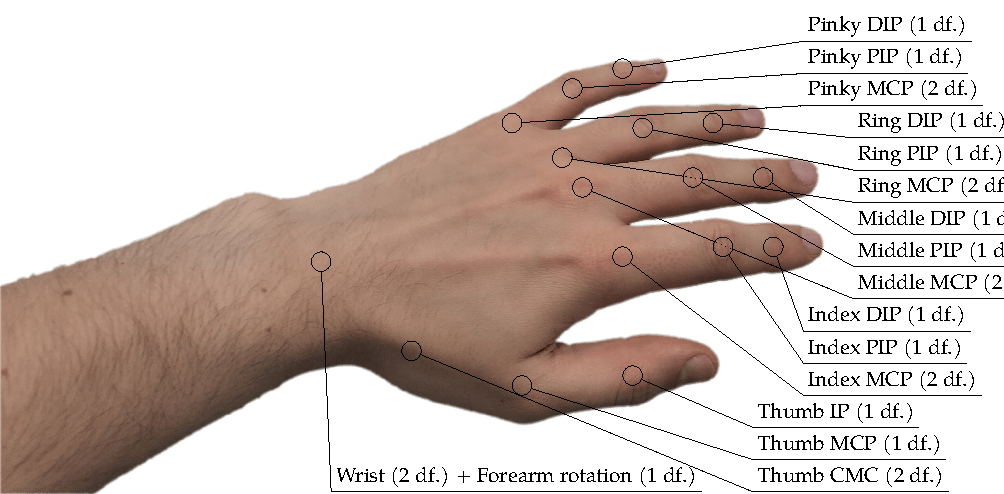
\includegraphics[width=1.1\linewidth]{figures/hand-joints.pdf}
    \captionsetup{parskip=7pt}
    \caption[Joints of the hand]{Each hand has 16 joints - three per digit, plus the wrist.

    The wrist and the first joint on each digit (the metacarpophalangeal (MCP) joints) can rotate on two axes, and so each have 2 degrees of freedom. The rest (the proximal- and distal-interphalangeal (PIP \& DIP) joints) can only rotate on one axis, and have 1.

    This naive counting gives 22 degrees of freedom. In addition, we usually consider rotation of the forearm (about the longitudinal axis) to be part of the hand, modeling it as a third degree of freedom of the wrist, which brings the total to 23 degrees of freedom.

    23 degrees of freedom is only a first approximation. A fully-realistic hand model needs to account for more minor degrees of freedom, such as deformation of the palm (movement of the metacrapal bones), minor rotation of the digits around their 3rd (length) axis, and movement of the skin and muscles. }
    \label{fig:hand-joints}
\end{figure}

It is not so straightforward to assign an angle to each of those 23 degrees of freedom. There are a variety of different parameterizations of the joints we might choose from, and additionally we have the option of placing constraints on the range of values that the angles can take. In this section we will discuss some of the most common parameterizations, and the pros and cons of each.

\clearpage

\subsection{Hierarchy of Rotations}

The most common parameterization of the hand is to use a hierarchy of rotations. Each joint is represented as a rotation (using one of the representations discussed in the previous section), along with an position offset, both relative to the previous joint. The magnitude of the offset typically remains fixed, because it represents the length of the bone. The wrist rotation is a rotation relative to the reference frame of the forearm (or the global reference frame, if only the hands are being modeled). The pinky MCP rotation is relative to the reference frame of the wrist, the PIP is relative to the MCP and so on. This means that rotating the wrist will change the position of all the joints in the hand, and rotating the MCP will change the position of all the joints below it, etc.

The benefit of this parameterization are that it matches the real kinematics of the hand -- rotating the wrist does in fact change the position of all the joints in the hand. For this reason this parameterization is used for the experiments in \Cref{C:hand-model}.

\subsection{Constraints}

Rather than representing each joint with a full rotation, we can place constraints on the range of values that the rotation can take. For example, the following constraints are used by \cite{hand-constraints}:
\begin{align}
\label{eqn:constraints}
\begin{aligned}
    0° ≤ \theta_{\text{MCP-F}} ≤ 90° \\
    -15° ≤ \theta_{\text{MCP-AA}} ≤ 15° \\
    0° ≤ \theta_{\text{PIP}} ≤ 110° \\
    0° ≤ \theta_{\text{DIP}} ≤ 90° \\
\end{aligned}
\end{align}

Whether or not to place constraints on the motion depends on the domain. For example, if we are modeling the hand for a virtual reality application, we might want to constrain the motion to be realistic. However, if we are training a neural network, then we cannot place non-differentiable constraints on the data, and it is more common to simply allow the network learn the constraints from the data.

\subsection{Point Cloud Representation}

For different tasks, different paramterizations might be appropriate. Take for example \textit{pose estimation}, where the task is to find the position and rotation of the joints from an image or video. In this case, a point cloud representation is often used, where each joint is represented by a point in 3D space. The benefit of this representation is that it is very easy to estimate from an image or video, and it is also easy to interpolate between two configurations. To then use this representation for animation, it is then converted into the hierarchical representation.


\section{Loss functions for learning angles}

\Cref{C:background} introduced some loss functions such as the Mean Squared Error (MSE) (\Cref{ss:mse}), which trains the model to output the posterior expectation $\mathbb{E}(y | x)$, and the Gaussian negative-log-likelihood which trains the model to output the posterior distribution $N(y | \mu, \sigma)$. This section will discuss some related loss functions that are used when data sits on a manifold, such as angles on the unit circle $S^1$, or rotations on $S^3$.
\subsection{Arc distance loss}
\label{ss:arc-dist}

The most obvious loss function that we might use when training a model to output angles is the arc distance between two angles. This is the distance between the two angles on the unit circle, and is given by
\begin{align}
\label{eqn:arc-dist}
\begin{aligned}
    \mathcal{L}_{\text{arc}}(y, \hat{y}) &= \cos^{-1}(\cos(y - \hat{y}))
\end{aligned}
\end{align}
A graph of this loss function is shown in \Cref{fig:loss-arc}. The loss is zero when the two angles are equal, and increases linearly as the angles move further apart. This loss function is not differentiable at $y = \hat{y} + \pi$, but this is not a problem because the model will never output this value.


\subsection{Angular mean squared error loss}
\label{ss:amse}

The analogous loss functions to the mean squared error for data that sits on the unit circle is the \textit{angular} mean-squared-error (eg. \cite{circ-statistics}), which will be used later on in \Cref{C:hand-model}. It is defined as follows:
\newcommand{\amse}{\mathcal{L}_{\theta\text{-MSE}}}
\begin{align}
\label{eqn:amse}
\begin{split}
    \fdef{\amse}{\R^{N×D}×\R^{N×D}}{\R} \\
    \amse&(Y, \hat{Y})_{ni} ≝ \frac{1}{N} \sum_{n, i} (\sin Y_{ni} - \sin \hat{Y}_{ni})^2 + (\cos Y_{ni} - \cos \hat{Y}_{ni})^2
\end{split}
\end{align}
where $Y$ and $\hat{Y}$ are sequences of vectors of angles, with batch shape $N$ and vector length $D$. We can see that the definition is similar to that of the circular mean in \Cref{ss:circ-mean}. A graph of the angular mean squared error loss is shown in \Cref{fig:loss-amse}.

\begin{figure}
    \centering
    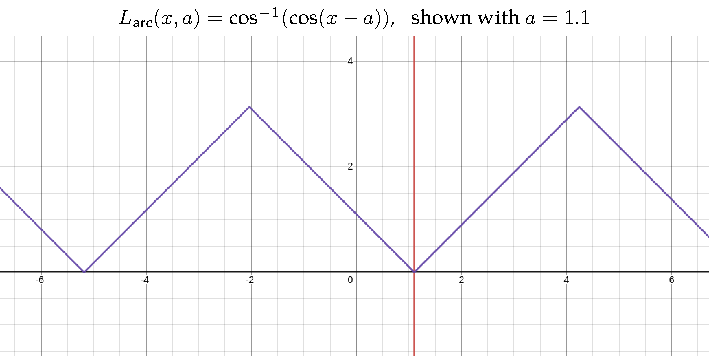
\includegraphics[width=0.9\linewidth]{figures/loss-arc.pdf}
    \captionsetup{parskip=7pt}
    \caption[Arc distance loss]{The arc distance loss function is the distance between two angles on the unit circle, analogous to the absolute distance for unbounded variables. It is zero when the two angles are equal, and increases linearly as the angles move further apart. The function is not differentiable at $y = \hat{y}$ and $y = \hat{y} + \pi$.}
    \hrulefill
    \label{fig:loss-arc}
\end{figure}
\begin{figure}
    \centering
    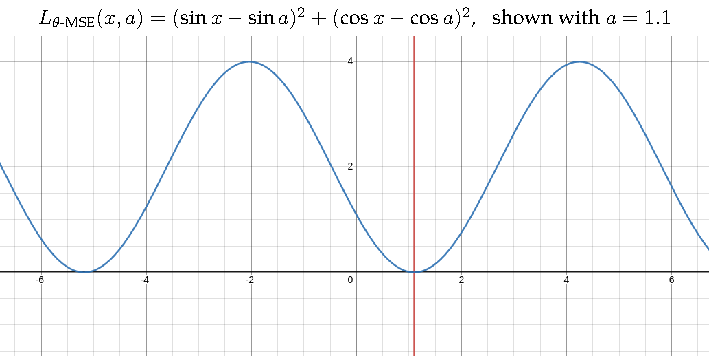
\includegraphics[width=0.9\linewidth]{figures/loss-amse.pdf}
    \captionsetup{parskip=7pt}
    \caption[Angular mean squared error loss]{The angular mean squared error loss function is analogous to the squared error for unbounded variables. It is zero when the two angles are equal, and increases quadratically as the angles move further apart, reaching a maximum when the two angles are opposite. Unlike the arc distance loss, the angular mean squared error loss is differentiable everywhere.}
    \label{fig:loss-amse}
\end{figure}

\clearpage


\subsection{Motivation for the Angular Mean Squared Error}
\label{ss:amse-motivation}

The angular mean squared error defined above in \Cref{ss:amse} is not arbitrarily chosen - it is the Maximum Likelihood Estimator (MLE) for the von-Mises distribution (the circular analogue of the Gaussian). The motivation and derivation for it is described in this subsection. First, for context, the derivation of the mean-squared-error from the likelihood function of the Gaussian distribution is given, and then the derivation of the angular mean-squared-error from the likelihood function of the von-Mises distribution.

As introduced in \Cref{ss:von-mises}, the von-Mises distribution is a distribution over angles on the unit circle. The Gaussian distribution and the von-Mises distribution are the \textit{maximum entropy} distributions of their respective domains. This means among all distributions over the real line $x \in (-\infty, \infty)$ with finite mean $\mu$ and variance $\sigma^2$, the Gaussian distribution $N(x \mid \mu, \sigma)$ is the one with the largest entropy. Similarly, among all distributions over the unit circle $x \in (-\pi, pi]$ with circular mean $\mu$ and circular variance $\kappa$, the von-Mises distribution is the one with the largest entropy.

As a result of this fact, training a model which outputs only a mean estimate with a mean-squared-error loss is equivalent to maximizing the likelihood of the data under the Gaussian distribution.

The likelihood function of a Gaussian distribution is as follows, where the mean $\mu$ is the output of the model $f(x, \theta)$.
\begin{align}
\label{notation:gaussian-likelihood}
\begin{aligned}
    \fdef{\mathbb{L}_G}{\R^P}{\R} \\
    \mathbb{L}_G&(\theta) ≝ \prod_n \frac{1}{\sqrt{2\pi\sigma^2}} \exp\left( -\frac{1}{2\sigma^2} (y_n - f(x_n, \theta))^2 \right)
\end{aligned}
\end{align}
where $x$ and $y$ are the input and target data respectively, $N$ is the number of data points, and $P$ is the number of parameters. For simplicity this is defined for scalar data, but the definition can be extended to vector data.

The optimization of the parameters $\theta$ is represented with the $\arg \max$ operator, which returns the value of $\theta$ that maximizes the likelihood of the data. Let $x$ and $y$ be the input and target data respectively, $N$ be the number of data points, and $P$ be the number of parameters.

The derivation is as follows:
\begin{align}
\label{eqn:gaussian-likelihood}
\begin{aligned}
    &\arg \max_\theta \mathbb{L}_G(\theta) \\
    = &\arg \max_\theta \prod_n \frac{1}{\sqrt{2\pi\sigma^2}} \exp\left( -\frac{1}{2\sigma^2} (y_n - f(x_n, \theta))^2 \right) \\
    = &\arg \max_\theta \prod_n \exp\left( -\frac{1}{2\sigma^2} (y_n - f(x_n, \theta))^2 \right) &&\text{by monotonicity} \\
    = &\arg \max_\theta \prod_n \exp\left( - (y_n - f(x_n, \theta))^2 \right) &&\text{by monotonicity} \\
    = &\arg \max_\theta \sum_n - (y_n - f(x_n, \theta))^2 &&\text{by monotonicity of} \ln \\
    = &\arg \min_\theta \sum_n (y_n - f(x_n, \theta))^2 \\
    = &\arg \min_\theta \frac{1}{N} \sum_n (y_n - f(x_n, \theta))^2 &&\text{by monotonicity} \\
    = &\arg \min_\theta \mse(y, f(x, \theta))
\end{aligned}
\end{align}

Similarly to the relationship between $\mse$ and the Gaussian, minimizing the angular mean-squared-error loss is equivalent to maximizing the likelihood of a von-Mises distribution. The likelihood function of a von-Mises distribution is as follows, where the circular mean $\mu$ is the output of the model $f(x, \theta)$.
\begin{align}
    \label{notation:von-mises-likelihood}
    \begin{aligned}
        \fdef{\mathbb{L}_\text{vM}}{\R^P}{\R} \\
        \mathbb{L}_\text{vM}&(\theta) ≝ \prod_n \frac{1}{2\pi I_0(\kappa)} \exp\left( \kappa \cos(y_n - f(x_n, \theta)) \right)
    \end{aligned}
\end{align}
where $x$ and $y$ are the input and target data respectively, $N$ is the number of data points, and $P$ is the number of parameters.
Again, for simplicity this is defined for scalar data, but the definition can be extended to vectors of angles.

Maximizing the above likelihood function is equivalent to minimizing the angular mean-squared-error loss. The derivation is as follows:
\begingroup
\allowdisplaybreaks
\begin{align*}
&\arg \max_{\theta} \mathbb{L}_\text{vM}(\theta) \\
= &\arg \max_{\theta} \prod_n \frac{1}{2\pi I_0(\kappa)} \exp\left( \kappa \cos(y_n - f(x_n, \theta)) \right) \\
= &\arg \max_{\theta} \prod_n \exp\left( \kappa \cos(y_n - f(x_n, \theta)) \right) &&\text{by monotonicity} \\
= &\arg \max_{\theta} \prod_n \exp\left( \cos(y_n - f(x_n, \theta)) \right) &&\text{by monotonicity} \\
= &\arg \max_{\theta} \sum_n \cos(y_n - f(x_n, \theta)) &&\text{by monotonicity of} \ln \\
= &\arg \min_{\theta} \sum_n - \cos(y_n - f(x_n, \theta)) \\
= &\arg \min_{\theta} \sum_n - \cos(y_n - f(x_n, \theta)) + 1 + 1 \\
= &\arg \min_{\theta} \sum_n - \cos(y_n - f(x_n, \theta)) + (\sin^2 y_n + \cos^2 y_n) \\
    &+ (\sin^2 f(x_n, \theta) + \cos^2 f(x_n, \theta)) &&\text{by} \sin^2 a + \cos^2 a = 1 \\
= &\arg \min_{\theta} \sum_n - (\sin y_n \sin f(x_n, \theta) + \cos y_n \cos f(x_n, \theta)) \\
    &+ (\sin^2 y_n + \cos^2 y_n) + (\sin^2 f(x_n, \theta) + \cos^2 f(x_n, \theta)) &&\begin{aligned}\text{by} &\cos(a ± b) \\ = &\cos a \cos b ∓ \sin a \sin b \end{aligned} \\
= &\arg \min_{\theta} \sum_n (\sin^2 y_n - \sin y_n \sin f(x_n, \theta) + \sin^2 f(x_n, \theta)) \\
    &+ (\cos^2 y_n - \cos y_n \cos f(x_n, \theta) +  \cos^2 f(x_n, \theta)) \\
= &\arg \min_{\theta} \sum_n (\sin^2 y_n + 2 \sin y_n \sin f(x_n, \theta) + \sin^2 f(x_n, \theta)) \\
    &+ (\cos^2 y_n + 2 \cos y_n \cos f(x_n, \theta) + 2 \cos^2 f(x_n, \theta)) &&\text{by monotonicity} \\
= &\arg \min_{\theta} \sum_n (\sin^2 y_n - 2 \sin y_n \sin f(x_n, \theta) + \sin^2 f(x_n, \theta)) \\
    &+ (\cos^2 y_n - 2 \cos y_n \cos f(x_n, \theta) + \cos^2 f(x_n, \theta)) \\
= &\arg \min_{\theta} \sum_n (\sin y_n - \sin f(x_n, \theta))^2 \\
    &+ (\cos y_n - \cos f(x_n, \theta))^2 \\
= &\arg \min_{\theta} \amse(y_n, \sin f(x_n, \theta)) \numberthis \label{eqn:amse-von-mises-derivation}
\end{align*}
\endgroup
